\subsection{基于语段关系/范式关系的模型}
\label{subsec:syntag-paradig}

\begin{figure}
  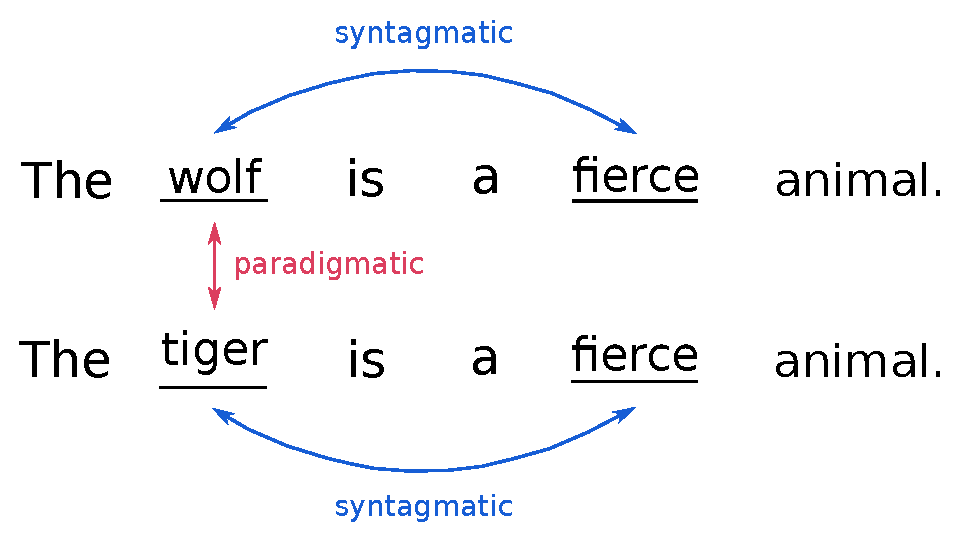
\includegraphics[width=0.6\textwidth]{figures/syntagmatic-model.eps}
  \centering
  \caption{语段和范式关系的例子\cite{pmlr-v22-bordes12}}
  \label{fig:syntagmatic-model}
\end{figure}

\subsubsection{语段关系与范式关系}
文集中可以利用的分布式信息有
语段关系(syntagmatic relation)和范式关系(paradigmatic
relation)两种\cite{Sahlgren2008}。
语段关系是指出现在相同文段(text region)的词的关系,如 \cref{fig:syntagmatic-model} 中,
wolf和fierce具有语段关系,因为它们出现在同一个句子中;
范式关系是指虽然不出现在同一个文段,但是拥有相似的上下文的词的关系,如
\cref{fig:syntagmatic-model} 中,tiger和wolf具有范式关系,因为它们
出现在相似的上下文中。根据所利用的分布式信息的不同,词向量模型可分为
基于语段关系和基于范式关系的模型。

\subsubsection{基于语段的模型}
基于语段的文献及其特点如 \cref{tab:syntag-models} 所示,
这些模型一般利用词--文档共现矩阵的信息。
由于具有相似含义的词倾向于出现在相似的文档中,如果我们观察词--文档共现矩阵,
就会发现含义相似的词,它们的行向量也较为接近\footnote{基于cosine相似度}。
在如 \cref{tab:word-doc} 所示的词--文档共现矩阵中,
词$w_3$和词$w_4$具有相似的行向量(cosine相似度为0.71),这表明它们存在语段关系。

\begin{table}
  \centering
  \caption{基于语段关系的模型}
  \label{tab:syntag-models}
  \begin{tabular}{ll}
    \toprule
    文献 & 特点 \\
    \midrule
    \cite{doi:10.1080/01690969108406936}
    \cite{DBLP:journals/cacm/RubensteinG65} & 使用句子作为文段 \\
    \cite{DBLP:journals/jasis/DeerwesterDLFH90} & 对词--文档共现矩阵采用了奇异值分解 \\
    \cite{lee99} & 对词--文档共现矩阵采用了正定矩阵分解 \\
    \bottomrule
  \end{tabular}
\end{table}

\begin{table}
  \setlength{\tabcolsep}{8pt}
  \centering
  \caption{词--文档共现矩阵\cite{Sahlgren2008}}
  \label{tab:word-doc}
  \begin{tabular}{|c|cccccccc|}
    \hline
    \multirow{2}{*}{Word} & \multicolumn{8}{c|}{Documents} \\
                          & 1 & 2 & 3 & 4 & 5 & 6 & 7 & 8  \\
    \hline
    $w_1$ & 0 & 1 & 0 & 0 & 0 & 0 & 0 & 0  \\
    $w_2$ & 0 & 0 & 1 & 0 & 0 & 3 & 0 & 0  \\
    $w_3$ & 1 & 0 & 0 & 2 & 0 & 0 & 5 & 0  \\
    $w_4$ & 3 & 0 & 0 & 1 & 1 & 0 & 2 & 0  \\
    $w_5$ & 0 & 1 & 3 & 0 & 1 & 2 & 1 & 0  \\
    $w_6$ & 1 & 2 & 0 & 0 & 0 & 0 & 1 & 0  \\
    $w_7$ & 0 & 1 & 0 & 1 & 0 & 1 & 0 & 1  \\
    $w_8$ & 0 & 0 & 0 & 0 & 0 & 7 & 0 & 0  \\
    \hline
  \end{tabular}
\end{table}

\subsubsection{基于范式的模型}
\begin{table}
  \centering
  \caption{词--词共现矩阵\cite{Sahlgren2008}}
  \label{tab:word-word}
  \begin{tabular}{|c|cccccccc|}
    \hline
    \multirow{2}{*}{Word} & \multicolumn{8}{c|}{Co-occurents} \\
                          & where & one & cannot & speak & thereof & must & be & silent  \\
    \hline
    where   & 0 & 1 & 0 & 0 & 0 & 0 & 0 & 0  \\
    one     & 0 & 0 & 1 & 0 & 0 & 1 & 0 & 0  \\
    cannot  & 0 & 0 & 0 & 1 & 0 & 0 & 0 & 0  \\
    speak   & 0 & 0 & 0 & 0 & 1 & 0 & 0 & 0  \\
    thereof & 0 & 1 & 0 & 0 & 0 & 0 & 0 & 0  \\
    must    & 0 & 0 & 0 & 0 & 0 & 0 & 1 & 0  \\
    be      & 0 & 0 & 0 & 0 & 0 & 0 & 0 & 1  \\
    silent  & 0 & 0 & 0 & 0 & 0 & 0 & 0 & 0  \\
    \hline
  \end{tabular}
\end{table}

基于范式的模型一般利用词--词共现矩阵的信息。具有范式关系的两个词
有着相似的上下文,根据分布式假设,它们的含义也相近。例如在
句子where one cannot speak thereof must be silent的词--词共现矩阵中( \cref{tab:word-word} ),
where和one具有相同的行向量,所以具有范式关系。
在模型分类方面,凡是利用了词--词共现矩阵的模型都可以归为基于范式的模型。
显式利用范式信息的模型有:
Glo~Vec\cite{pennington2014glove},
超空间类比语言模型(HAL)\cite{lund95},
海灵格主成分分析法(HPCA)\cite{DBLP:conf/eacl/LebretC14}等。
隐式利用范式信息的模型有:
神经网络语言模型(NNLM)\cite{DBLP:journals/jmlr/BengioDVJ03},
\texttt{word2vec}模型\cite{DBLP:journals/corr/abs-1301-3781},
循环神经网络语言模型(RNNLM)\cite{DBLP:conf/interspeech/MikolovKBCK10}等。

\subsubsection{同时利用语段和范式关系的模型}
Fei Sun等人在\cite{DBLP:conf/acl/SunGLXC15}中提出了两个同时捕获语段和范式
关系的模型,分别为并行文档上下文模型(Parallel Document Context Model,PDC)和
分层文档上下文模型(Hierarchical Document Context Model,HDC)。
Fei Sun等人在\texttt{word2vec}模型的基础上加入了基于文档的预测分支,把CBOW扩展为PDC,把Skip-gram扩展为HDC。

\paragraph{模型体系结构}
\begin{figure}
  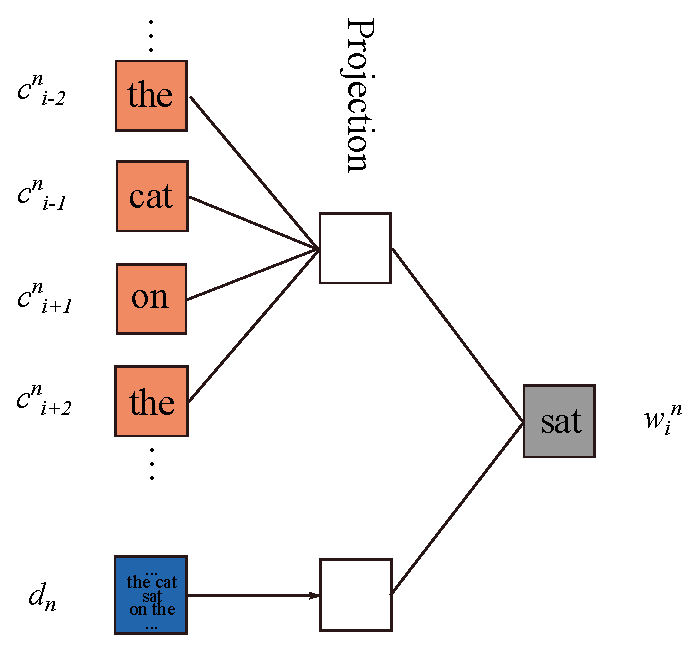
\includegraphics[width=0.6\textwidth]{figures/jointly-parallel-arch.eps}
  \centering
  \caption{PDC模型的体系结构\cite{DBLP:conf/acl/SunGLXC15}}
  \label{fig:jointly-pdc}
\end{figure}

PDC模型的体系结构如 \cref{fig:jointly-pdc} 所示。和CBOW一致的是,周围的词被用于预测目标词,以捕获范式信息;
词所在的文档也被用于预测目标词,以捕获了语段信息。
因为文档预测分支和上下文预测分支在预测目标词中处于并行的位置,所以称为并行文档上下文模型。

PDC模型的目标函数为:
\begin{align}
  l = \sum_{n=1}^N \sum_{w_i^n \in d_n}%
  \left( \log p(w_i^n|h_i^n) + \log p(w_i^n|d_n)\right)
  \label{eqn:jointly-pdc-objective}
\end{align}
其中$h_i^n$表示$w_i^n$的上下文的投影,定义为:
\begin{align}
  h_i^n = \frac{1}{L} \sum_{j=-L}^{L} c^n_j
  \label{eqn:jointly-pdc-context}
\end{align}

$p(w_i^n|h_i^n)$和$p(w_i^n|d_n)$定义为:
\begin{align}
  p(w_i^n|h_i^n) = \frac{\exp(\vec{w}_i^n \cdot \vec{h}_i^n)}%
  {\sum_{w\in W}\exp(\vec{w}\cdot\vec{h}_i^n)}
  \label{eqn:jointly-pdc-word}
\end{align}
\begin{align}
  p(w_i^n|d_n) = \frac{\exp(\vec{w}_i^n \cdot \vec{h}_n)}%
  {\sum_{w\in W}\exp(\vec{w}\cdot\vec{h}_n)}
  \label{eqn:jointly-pdc-doc}
\end{align}

\begin{figure}
  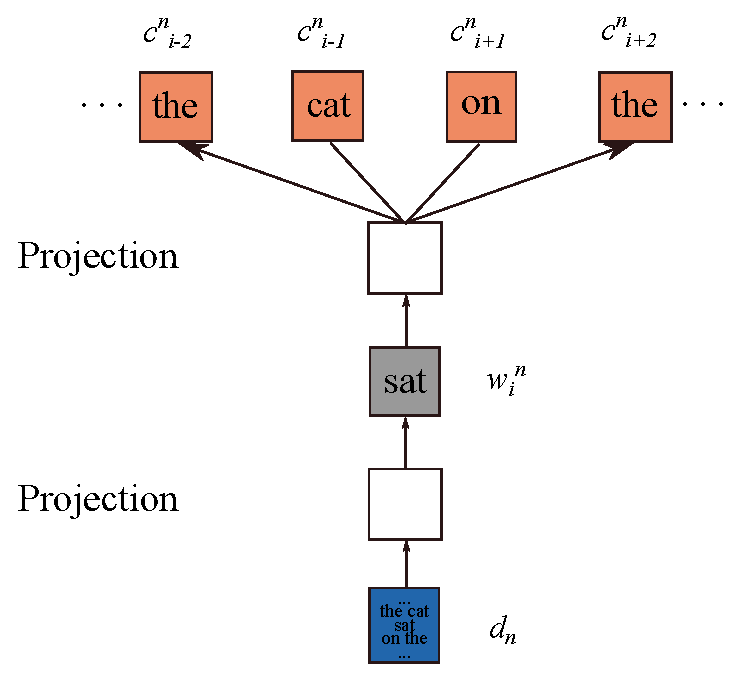
\includegraphics[width=0.6\textwidth]{figures/hierachical-model.eps}
  \centering
  \caption{HDC模型的体系结构\cite{DBLP:conf/acl/SunGLXC15}}
  \label{fig:jointly-hdc}
\end{figure}

HDC模型的体系结构如 \cref{fig:jointly-hdc} 所示。
该模型用词所在的文档预测一个目标词,然后用目标词预测它周围的词。
因为预测以分层的方式展开,该模型称为分层文档上下文模型。
类似于PDC模型,HDC通过文档预测分支学习语段关系,通过上下文预测分支学习范式关系。
HDC模型的目标函数为:
\begin{align}
  l = \sum_{n=1}^N \sum_{w_i^n \in d_n}%
  \left(\sum_{\substack{j=i-L\\ j \neq i}}^{i+L}%
  \log p(c_j^n|w_i^n)+\log p(w_i^n|d_n)\right)
  \label{eqn:jointly-hdc-objective}
\end{align}

其中,$p(w_i^n|d_n)$如\cref{eqn:jointly-pdc-doc}所定义;$p(c_j^n|w_i^n)$ 的定义如下:
\begin{align}
  p(c_j^n|w_i^n) = \frac{\exp(\vec{c}_j^n \cdot \vec{w}_i^n)}%
  {\sum_{c \in W} \exp(\vec{c} \cdot \vec{w}_i^n)}
  \label{eqn:jointly-hdc-word}
\end{align}

\paragraph{时间复杂度}
PDC和HDC模型作为预测型模型,整体的时间复杂度服从\cref{eqn:predict-based-complexity}。和分析\texttt{word2vec}的方法类似,我们给出$Q$。
对于PDC,$Q$为:
\begin{align}
  Q = D + N \times D + D \times \log_2(V)
  \label{eqn:jointly-pdc-complexity}
\end{align}
其中$N$为窗口大小,$D$为词向量的维度(也是文档向量的维度),
$V$为词汇表的大小。
对于HDC,$Q$为:
\begin{align}
  Q = C \times (2D + D \times \log_2(V))
  \label{eqn:jointly-hdc-complexity}
\end{align}
其中$C$是词的最大距离。

\paragraph{讨论}
优点:由于同时捕获了语段和范式关系,
这两个模型在词类比问题和相似度任务上均超过了CBOW,Skip-gram和Glo~Vec等基线模型。
缺点:模型增加了额外的文档预测分支和一个$K \times D$的文档矩阵参数,其中$K$为
文档的数量,$D$为向量的维度。
